\chapter{Background}
\section{Debugger internals}
Debuggers are an essential tool for software developers, as they allow us to pause the execution of a program and inspect its state at any given moment. This is useful for detecting and fixing bugs, as well as for understanding how the program works. In this section, we will introduce some of the internals of debuggers, starting with the INT3 instruction.

The INT3 instruction, also known as the 0xcc byte, is used by debuggers to implement software breakpoints. When a debugger encounters this instruction in the program's code, it will pause the execution of the program and allow the user to inspect its state. This is useful for setting breakpoints at specific locations in the code, and for stepping through the program one instruction at a time.

Another important aspect of debugging is ASLR, or Address Space Layout Randomization. This is a security feature that randomizes the locations of certain parts of the program in memory, making it more difficult for attackers to exploit vulnerabilities. Debuggers must be able to decode the proc-maps file, which contains information about the locations of the various parts of the program, in order to properly interact with the program.

GDB, a popular command line debugger, implements a variety of features to make debugging easier. One feature that I found particularly interesting was how it understands the current stack trace.

GDB reads the stack trace by accessing the memory locations that store the stack frame pointers and function return addresses. The stack frame pointer is a register that points to the current stack frame, which contains the local variables and arguments for the current function. The function return address is the address of the next instruction to be executed when the current function returns.

By following the sequence of stack frame pointers and function return addresses, gdb can reconstruct the sequence of function calls that led to the current point in the program's execution. This information is then displayed to the user in the form of a stack trace, which shows the names and arguments of the functions that were called.

There is a lot to say about debugger internals, but this should be enough information to understand the rest of this paper. 

\section{State Diagrams}
State diagrams, also known as finite state machines (FSM), are a useful tool in the realm of debugging. They provide a visual representation of the possible states of a program and the transitions between them.

Each node in a state diagram represents a unique state of the program. These states can be thought of as the different possible ways that the program can behave. For example, in a simple program that takes user input, there may be a "waiting for user input" state and a "processing user input" state.

Transitions between these states are represented by edges on the state diagram. These transitions are triggered by certain events or actions within the program. For example, in our simple program, the transition from the "waiting for user input" state to the "processing user input" state would be triggered by the user entering input.

Flow control within the program can be easily visualized and understood through the use of state diagrams. For instance, in the case of a conditional statement, the state diagram would split into multiple branches depending on the outcome of the conditional.

\begin{figure}
\centering
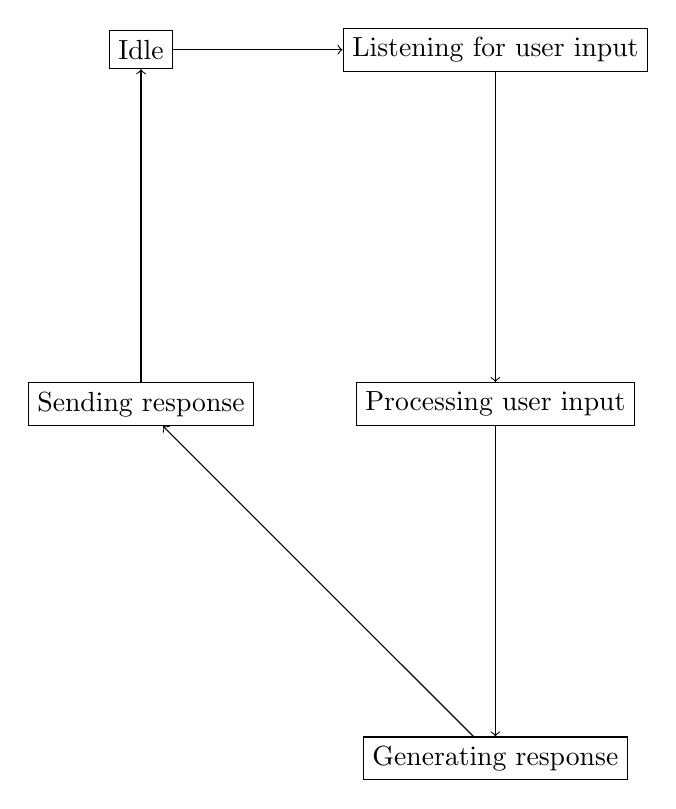
\begin{tikzpicture}[node distance=4.5 cm]
\node[rectangle, draw] (A) {Idle};
\node[rectangle, draw] (B) [right of=A] {Listening for user input};
\node[rectangle, draw] (C) [below of=B] {Processing user input};
\node[rectangle, draw] (D) [below of=C] {Generating response};
\node[rectangle, draw] (E) [left of=C] {Sending response};
\draw [->, =>stealth] (A) -- (B);
\draw [->, =>stealth] (B) -- (C);
\draw [->, =>stealth] (C) -- (D);
\draw [->, =>stealth] (D) -- (E);
\draw [->, =>stealth] (E) -- (A);
\end{tikzpicture}
\caption{Simple state diagram for a bot}
\end{figure}

This state diagram provides a clear visual representation of a generic bot's behavior, allowing developers to easily understand how the program is executing and how it will respond to different inputs. State diagrams are particularly useful for onboarding new developers, as they provide a high-level overview of the program's flow without requiring a deep understanding of the code.


\section{ELF / DWARF}
The ELF (Executable and Linkable Format) is a file format used by many Unix-like operating systems to specify the layout of object files and executables. These files contain a wealth of information about the compiled code, including symbols, debugging information, and other metadata.

One component of ELF files is DWARF (Debugging With Attributed Record Formats), which is a debugging data format that specifies the format of debugging information. DWARF data is embedded in ELF files and can be accessed by debuggers, such as gdb, to provide valuable information about the execution of a program.

DWARF data is organized into structures called DIEs (Debugging Information Entries), which contain tags identifying the type of information they contain. Some common DIE tags include DW\_TAG\_variable for variables, DW\_TAG\_subprogram for functions, and DW\_TAG\_compile\_unit for compilation units. \\

\begin{table}
\centering
\begin{tabular}{|c|c|}
\hline
\textbf{Attribue} & \textbf{Description} \\ \hline
DW\_AT\_name & The name of the subprogram \\ \hline
DW\_AT\_low\_pc & The starting address of the subprogram \\ \hline
DW\_AT\_high\_pc & The ending address of the subprogram \\ \hline
DW\_AT\_decl\_file & The file in which the subprogram is declared \\ \hline
DW\_AT\_decl\_line & The line on which the subprogram is declared \\ \hline
DW\_AT\_prototyped & Specifies whether the subprogram has a prototype \\ \hline
\end{tabular}
\caption{A table of attributes for a DW\_TAG\_subprogram DIE.}
\end{table}

By parsing out these DIE tags, debuggers can access valuable information about the symbols in a program, allowing them to provide useful features such as the ability to inspect and modify variables during execution.

In the context of my live-debugger, Execumap, DWARF data plays a crucial role in my ability to create a state-diagram of the program's execution. By accessing and parsing DWARF data from the recorded trace, I am able to identify the symbols and their relationships in the program.

\section{RR Record and Replay Framework}
The rr record and replay framework is a powerful tool for debugging programs. It allows users to record a program's execution and then replay it at a later time. This allows users to easily and quickly reproduce the conditions that led to a bug. This is particularly useful when debugging rare or timing-sensitive bugs like race conditions where gdb might prevent the bug from ever occuring in the first place.

One key aspect of rr is its focus on capturing nondeterministic input rather than the whole trace \cite{rr-site}. In this case, nondeterministic input are the events that could cause a program's output to vary from run to run. This includes things like syscalls, process-switching timings, or even some non-deterministic instructions. By capturing and replaying these inputs, rr avoids having to walk through and instrument the vast majority of executed instructions. To accomplish this, rr uses a wide variety of tools, including the `ptrace` interface to attach middleware, overwriting the the vDSO (virtual dynamic shared object), limiting a program to a single core, and other more specific techniques. 

To intercept many simple system calls, rr can simply overwrite the vDSO which is a use-space code-segement that the kernel exports for code "that does not necessarily have to run in kernel space" \cite{vdso} However some code directly calls syscalls. As such, "when the tracee makes a system call, RR is notified via a ptrace rap and it tries to rewrite the system-call instruction to call into [their] interception library" \cite[p.~8]{rr}. A diagram of this modification can be seen in figure 2.2. 

(TODO)
During the replay phase, rr uses this information to replay the system call, allowing the program to execute as if the original system call had been made. This allows rr to accurately reproduce the program's execution, including any system calls that were made. 
(TODO)

\begin{figure}
\centering
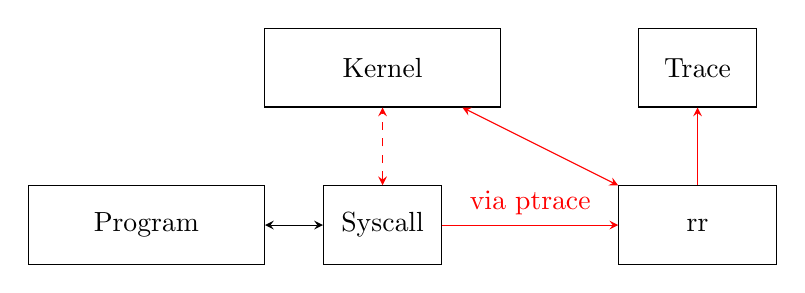
\begin{tikzpicture}

%RR
\node[rectangle, draw, minimum width=2cm, minimum height=1cm] (rr) at (7,-2) {rr};

%Kernel
\node[rectangle, draw, minimum width=3cm, minimum height=1cm] (kernel) at (3,0) {Kernel};

%Program
\node[rectangle, draw, minimum width=3cm, minimum height=1cm] (program) at (0,-2) {Program};

%VDSO
\node[rectangle, draw, minimum width=1.5cm, minimum height=1cm] (syscall) at (3,-2) {Syscall};

%Trace
\node[rectangle, draw, minimum width=1.5cm, minimum height=1cm] (trace) at (7,0) {Trace};

%System Call
\draw[<->, >=stealth] (program) -- (syscall);
\draw[<->, >=stealth, red, dashed] (syscall) -- (kernel);
\draw[<->, >=stealth, red] (rr) -- (kernel);
\draw[->, >=stealth, red] (syscall) -- (rr) node[midway,above ] {via ptrace};
\draw[->, >=stealth, red] (rr) -- (trace);

\end{tikzpicture}
\caption{Diagram showing how rr intercepts calls into the kernel and records them}
\end{figure}
    In order to efficently "continue-backwards", rr utilizes a checkpointing system. The checkpointing system works by \begin{verbatim}fork\end{verbatim}ing the process to cheaply copy the address space \cite[p.~15]{rr}. This is efficient because "fork is (mostly) 'copy-on-write' and is very well optimized on Linux, so creating a checkpoint typically takes less than ten milliseconds." \cite[p.~15]{rr}. This allows rr to quickly and easily restore the program to the state it was in at the time of the checkpoint during the replay phase. Then it can "continue-forwards" until it reaches the desired location.

The default interface to rr is a gdb server using the gdb messaging protocol. However, this is not a performant solution for a programmatic interface that might be doing queries across the entire execution of a program. As such, we developed librr, a Rust library to interact with the C++ internals and provide nice abstractions such as reading registers, writing bytes in memory, setting breakpoints, etc. 

Execumap uses RR (and librr) extensively and would not be possible without them. The ability to gather more information about a programs execution after it happened is has been useful as I am not able to predict all of the locations that a user might want to visit. Similarly, without these tools I would be unable to allow the user to open up the trace to any location within the program's execution.


